\documentclass{beamer}
\usetheme{pnl}
\usepackage[utf8]{inputenc}
\usepackage[T1]{fontenc}
\usepackage{hyperref}
\usepackage{tikz}
\usetikzlibrary{positioning}

\graphicspath{{img/}}

\title{Practice Big Data-NET17237}
\date[8-9-2022]{Instalasi}
\author[Davi]{Muhammad Davi, S.Kom., M.Cs.\\ \texttt{muhammad.davi@pnl.ac.id}\\ 
\texttt{\small 14-9-\the\year{}}}

\begin{document}

\tikzset{
	phase/.style={draw,minimum width=1cm,minimum height=1cm,align=center},
	previous/.style={below right=0.1cm of #1}
}
  
\newcommand\connect[2]{
	\draw[->,thick] (#1) -| (#2);
	\draw[->,thick] (#2) -| (#1);
}
  
\begin{frame}[t]
\titlepage
\end{frame}

\begin{frame}[t]
\frametitle{Outline}
\begin{itemize}
\item Install Java
\item Install Hadoop
%\item Konfigurasi Hadoop dan Java
\item Running Hadoop
\end{itemize}
\end{frame}

\begin{frame}[t]
\frametitle{Install Java}
\framesubtitle{Instalasi}
\begin{itemize}
\item Install Java
\begin{itemize}
\item sudo apt update
\item sudo apt install openjdk-8-jdk -y
\end{itemize}
\item Verifikasi Java
\begin{itemize}
\item java -version
\end{itemize}
\end{itemize}
\end{frame}

\begin{frame}[t]
\frametitle{Install Hadoop}
\framesubtitle{Instalasi}
\begin{itemize}
\item Buat folder
\begin{itemize}
\item mkdir $\sim$/hadoop
\end{itemize}
\item Pindah ke folder hadoop
\begin{itemize}
\item cd hadoop
\end{itemize}
\item Download Hadoop \href{https://hadoop.apache.org/releases.html}{(https://hadoop.apache.org/releases.html)}
\begin{figure}
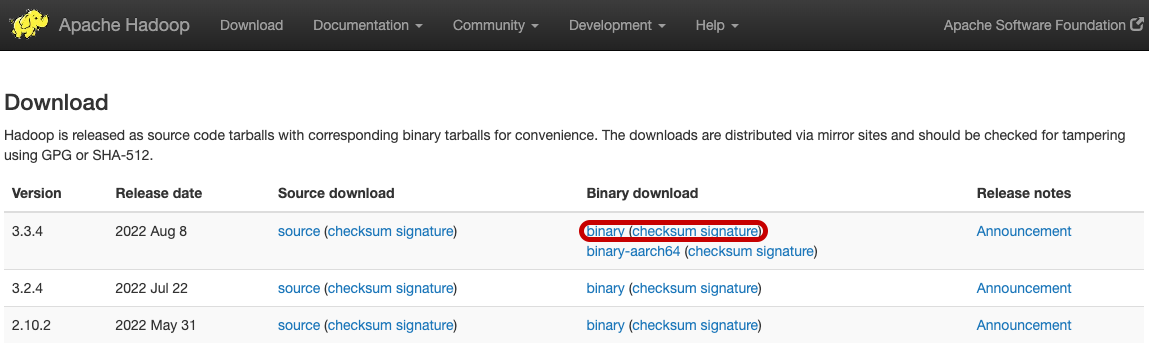
\includegraphics[scale=.25]{download-hadoop-1.png}
\end{figure}
\end{itemize}
\end{frame}

\begin{frame}[t]
\frametitle{Running Hadoop}
\framesubtitle{Instalasi}
\begin{itemize}
\item /usr/local/hadoop/bin/hadoop
\end{itemize}
\end{frame}

%thank you
\setbeamertemplate{background}{}
\setbeamertemplate*{lastpage}{}
\usebeamertemplate*{lastpage}

\end{document}
